%%% Décommenter pour une présentation
\documentclass{beamer}
%%%

%%% Décommenter pour avoir un article
%\documentclass[handout]{beamer}
%\usepackage{pgfpages}
%\pgfpagesuselayout{2 on 1}[a4paper,border shrink=5mm]
%\setbeameroption{show notes on second screen=bottom} % Beamer manual, section 19.3
%%%

%%%%%%%%%%%%%%%%%%%%%%%%%%%%%%%%%%%%%%%%%%%%%%%%%%%%%%%%%%%%%%%%%%%%%%
% NE PAS MODIFIER CETTE PARTIE

\usetheme{Warsaw}
\usepackage[utf8]{inputenc}
\usepackage[T1]{fontenc}
\usepackage{amsmath}
\usepackage{amsfonts}
\usepackage{amssymb}
\usepackage{graphicx}
\usepackage{listings}
\usepackage{hyperref}
\usepackage{tikz}
\usepackage{verbatim}
\usepackage{algorithm}
\usepackage{algorithmic}
\usetikzlibrary{arrows,shapes}

\graphicspath{{graphics/}}

\hypersetup{pdfstartview={Fit}}



\AtBeginSection[]{
  \begin{frame}
  \vfill
  \centering
  \begin{beamercolorbox}[sep=8pt,center,shadow=true,rounded=true]{title}
    \usebeamerfont{title}\insertsectionhead\par%
  \end{beamercolorbox}
  \vfill
  \end{frame}
}

\setbeamertemplate{note page}[plain] % Beamer manual, section 19.1
\newlength{\parskipbackup}
\setlength{\parskipbackup}{\parskip}
\newlength{\parindentbackup}
\setlength{\parindentbackup}{\parindent}
\newcommand{\baselinestretchbackup}{\baselinestretch}
\usetemplatenote{\rmfamily \scriptsize%
  \setlength{\parindent}{1em} \setlength{\parskip}{1ex}%
  \renewcommand{\baselinestretch}{1}%
  \noindent \insertnote%

  \setlength{\parskip}{\parskipbackup}%
  \setlength{\parindent}{\parindentbackup}%
  \renewcommand{\baselinestretch}{\baselinestretchbackup}%
}

\logo{
	
\includegraphics[scale=0.1]{SPCL.png}
} 
\institute[ETH Zürich]{\textbf{ETH Zürich}}




%%%%%%%%%%%%%%%%%%%%%%%%%%%%%%%%%%%%%%%%%%%%%%%%%%%%%%%%%%%%%%%%%%%%


%TODO : PARTIE A MODIFIER 

\date{December 2018}	

\author{
    Th. Cambier
    R. Dang-Nhu
    Th. Dardinier
    C. Trassoudaine
}
\title{
	\textbf{Minimum Spanning Tree}\\
	-\\ 
	\textit{DPHPC}
}

\usepackage[backend=biber, style=authoryear, doi=false,isbn=false,url=false, giveninits=true]{biblatex}
\bibliography{bib.bib}
 
\usepackage{mathrsfs}

\begin{document}

\pgfdeclarelayer{background}
\pgfsetlayers{background,main}

\frame{\titlepage}
\frame{\tableofcontents}

%%%%%%%%%%%%%%%%%%%%%%%%%%%%%%%%%%%%%%%%%%%%%%%%%%%%%%%%%%%%%%%%%%%%
% SECTION 1
%%%%%%%%%%%%%%%%%%%%%%%%%%%%%%%%%%%%%%%%%%%%%%%%%%%%%%%%%%%%%%%%%%%%


\section{Problem definition - reminder}
\subsection{The MST Problem}
\begin{frame}
\frametitle{The MST problem}
 A minimum spanning tree (MST) or minimum weight spanning tree is a subset of the edges of a connected, edge-weighted (un)directed graph that connects all the vertices together, without any cycles and with the minimum possible total edge weight. 
 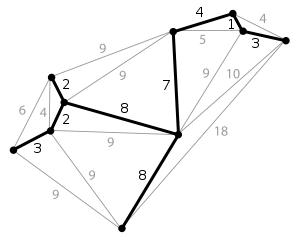
\includegraphics[width=.5\textwidth]{MST.png}
\end{frame}


\subsection{Use cases}

\begin{frame}
\frametitle{Input sets: $G(n,p)$}
\centering
$G(100, 0.02)$
\begin{figure}
 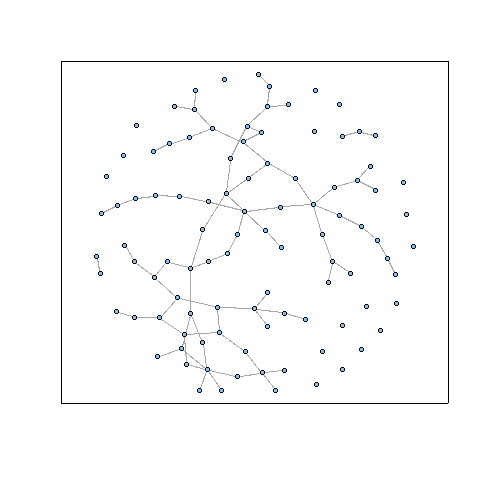
\includegraphics[width=.7\textwidth]{graphGNP.png}
\end{figure}
\end{frame}

\begin{frame}
\frametitle{Input sets: $PA(n)$}
\centering
$PA(100)$
\begin{figure}
 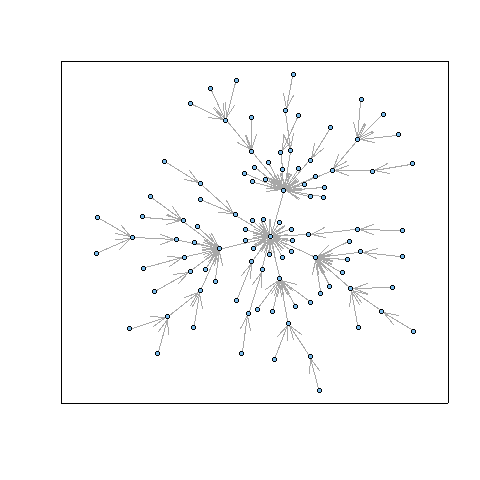
\includegraphics[width=.7\textwidth]{graphPA.png}
\end{figure}
\end{frame}

\begin{frame}
\frametitle{Input sets: 9\textsuperscript{th} DIMACS challenge dataset}
\centering
USA Roads
\begin{figure}
 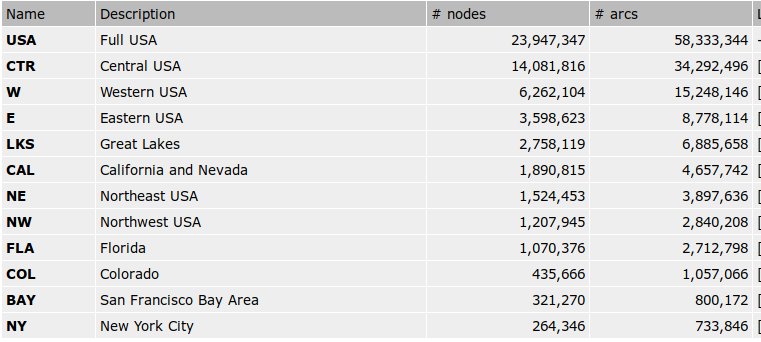
\includegraphics[width=.7\textwidth]{graphUSA.png}
\end{figure}
\end{frame}


\section{Algorithms and parallel implementations}

\subsection{Base serial algorithms}

\begin{frame}[fragile]
\frametitle{Sollin}
\small
\begin{algorithm}[H]
\begin{algorithmic}[1]

\STATE F = set(one-vertex trees)
\WHILE{$\mid F \mid > 1$}
\STATE TODO
\ENDWHILE

\end{algorithmic}
\end{algorithm}
\end{frame}

\begin{frame}[fragile]
\frametitle{Kruskal}
\small
\begin{algorithm}[H]
\begin{algorithmic}[1]
\STATE $A = \emptyset$
\FORALL{$v \in G.V$}
\STATE MAKE-SET$(v)$
\ENDFOR
\STATE Sort (asc.) $\left(weight(u, v)\right)_{(u, v) \in G.E}$
\FORALL{$(u, v)$ in $G.E$ ordered by weight}
\IF{FIND-SET$(u)$ $\neq$ FIND-SET$(v)$}
\STATE $A = A \cup {(u, v)}$
\STATE UNION$(u, v)$
\ENDIF
\ENDFOR
\RETURN A
\end{algorithmic}
\end{algorithm}


\end{frame}

\begin{frame}
\frametitle{Boost implementations}

\begin{columns}
\begin{column}{.7\linewidth}
\begin{itemize}
\item Boost-Kruskal used as a reference
\end{itemize}
\end{column}

\begin{column}{.3\linewidth}

\includegraphics[width=\linewidth]{boost.png}
\end{column}
\end{columns}

\end{frame}


\subsection{Parallel improvements}

\begin{frame}
\frametitle{Parallel sorting on Kruskal}

\end{frame}

\begin{frame}

	\frametitle{Filter Kruskal}

    $E$: set of edges, $m = |E|$, $p$ is the number of cores, $T(m)$ is the runtime with $m$ edges.

	\begin{enumerate}
        \item If $m \leq threshold$ then solve with Kruskal
        \item Find pivot for edges (weight)\only<2->{: $O(1)$}
            \only<2>{
                \begin{itemize}
                    \item Concurrently sample $256$ elements from the list (\textbf{OpenMP})
                    \item Sort the list and return the median (\textbf{TBB})
                \end{itemize}
            }
        \item Partition $E$ into $E_{\leq}, E_{>}$\only<3->{: $O\left(\frac{m}{p}\right)$}
            \only<3>{
                \begin{itemize}
                    \item Partition function (\textbf{Intel Parallel STL})
                \end{itemize}
            }
        \item $A_{\leq} = filterKruskal(E_{\leq})$\only<4->{: $T\left(\frac{m}{2}\right)$}
        \item $E_{>} = filter(E_{>})$\only<5->{: $ O\left( \frac{m}{p} \right) $}
            \only<5>{
                \begin{itemize}
                    \item Partition function (\textbf{Intel Parallel STL})
                \end{itemize}
            }
        \item $A_{>} = filterKruskal(E_{>})$\only<6->{: $O\left( T\left( \frac{m}{2} \right) \right)$}
            \only<6>{
                \begin{itemize}
                    \item In practice way less than $\frac{m}{2}$
                \end{itemize}
            }
        \item Return $merge(A_{\leq}, A_{>})$\only<7->{: $O(1)$}
    \end{enumerate}

\end{frame}

\begin{frame}

    \frametitle{Filter Kruskal: Complexity analysis}

    \begin{itemize}
        \item Worst case:
            $T(m) \leq O\left( \frac{m}{p} \right) + 2 T\left( \frac{m}{2} \right) $
            \\
            \only<2->{
                $T(m) = O\left( \frac{m \ln(m)}{p} + m \right) $
            }
        \item Best case:
            $T(m) \leq O\left( \frac{m}{p} \right) + T\left( \frac{m}{2} \right) $
            \\
            \only<3->{
                $T(m) = O\left( \frac{m}{p} + m \right)  = O(m)$
            }
        \only<4->{
            \item $O(m) \leq T(m) \leq O\left( \frac{m \ln(m)}{p} + m \right) $
        }
    \end{itemize}

\end{frame}

\begin{frame}
    \frametitle{Amdahl's law}

	$S_p$ is the speedup with $p$ cores, $f$ is the part of the program that is sequential.

	\[
		S_p = \frac{1}{\frac{1-f}{p} + f}
	\]
	\[
		f = \frac{\frac{p}{S_p} - 1}{p - 1}
	\]

\end{frame}

\begin{frame}

    \frametitle{Amdahl's law: Kruskal}

	Graph: Erdos-Renyi (100,000 nodes, $p=0.0005$)

	\begin{center}
		\begin{tabular}{||c c c c||} 
			\hline
            Cores & Median speed-up & Standard deviation & f \\ [0.5ex] 
			\hline\hline
            1 & 1 & 0.0129805395 & - \\
			\hline
            2 & 1.1881513396 & 0.0400305172 & 0.6832872491 \\
			\hline
            4 & 1.3340592415 & 0.0130798641 & 0.6661225318 \\
			\hline
            8 & 1.3134515984 & 0.01048841 & 0.7272602975 \\
			\hline
            16 & 1.4399618642 & 0.0088220116 & 0.6740936918 \\
			\hline
            32 & 1.3877640643 & 0.0442081933 & 0.7115701488 \\ [1ex] 
			\hline
		\end{tabular}
	\end{center}

\end{frame}

\begin{frame}

    \frametitle{Amdahl's law: Filter Kruskal}

	Graph: Preferential attachment (10,000 nodes, 1,000 edges per vertex)

	\begin{center}
		\begin{tabular}{||c c c c||} 
			\hline
            Cores & Median speed-up & Standard deviation & f \\ [0.5ex] 
			\hline\hline
			1 & 1 & 0.174182691 & - \\
			\hline
			2 & 1.6268639022 & 0.2472258016 & 0.2293591353 \\
			\hline
			4 & 2.669168898	& 0.5213238241 & 0.1661979381 \\
			\hline
			8 & 5.3584384444 & 0.9757941767 & 0.0704246098 \\
			\hline
			16 & 5.7447285937 & 1.108109986 & 0.1190108026 \\
			\hline
			32 & 5.6322979489 & 1.497976882 & 0.1510166972 \\ [1ex] 
			\hline
		\end{tabular}
	\end{center}

\end{frame}

\begin{frame}
\frametitle{Filter Sollin}

\end{frame}


\begin{frame}
    \printbibliography
\end{frame} 

\section{Results overview}

\subsection{Setup}

\begin{frame}
\frametitle{EULER Cluster}

\end{frame}

\subsection{Results}

\begin{frame}
\frametitle{Scalability}

\end{frame}

\begin{frame}
\frametitle{Speedups}

\end{frame}




\end{document}
